%----------
%   WARNING
%----------

% This Guide contains Library recommendations based mainly on APA and IEEE styles, but you must always follow the guidelines of your TFG Tutor and the TFG regulations for your degree.

% THIS TEMPLATE IS BASED ON THE IEEE STYLE 


%----------
% DOCUMENT SETTINGS
%----------

\documentclass[12pt]{report} % font: 12pt

% margins: 2.5 cm top and bottom; 3 cm left and right
\usepackage[
a4paper,
vmargin=2.5cm,
hmargin=3cm
]{geometry}

% Paragraph Spacing and Line Spacing: Narrow (6 pt / 1.15 spacing) or Moderate (6 pt / 1.5 spacing)
\renewcommand{\baselinestretch}{1.15}
\parskip=6pt

% Color settings for cover and code listings 
\usepackage[table]{xcolor}
\definecolor{azulUC3M}{RGB}{0,0,102}
\definecolor{gray97}{gray}{.97}
\definecolor{gray75}{gray}{.75}
\definecolor{gray45}{gray}{.45}

% PDF/A -- Important for its inclusion in e-Archive. PDF/A is the optimal format for preservation and for the generation of metadata: http://uc3m.libguides.com/ld.php?content_id=31389625. 

% In the template we include the file OUTPUT.XMPDATA. You can download that file and include the metadata that will be incorporated into the PDF file when you compile the memoria.tex file. Then upload it back to your project.  
\usepackage[a-1b]{pdfx}

% LINKS
\usepackage{hyperref}
\hypersetup{colorlinks=true,
	citecolor=black,
	linkcolor=black, % links to parts of the document (e.g. index) in black
	urlcolor=blue} % links to resources outside the document in blue

% MATH EXPRESSIONS
\usepackage{amsmath,amssymb,amsfonts,amsthm}

% Character encoding
\usepackage{txfonts} 
\usepackage[T1]{fontenc}
\usepackage[utf8]{inputenc}

% English settings
\usepackage[english]{babel} 
\usepackage[babel, english=american]{csquotes}
\AtBeginEnvironment{quote}{\small}

% Footer settings
\usepackage{fancyhdr}
\pagestyle{fancy}
\fancyhf{}
\renewcommand{\headrulewidth}{0pt}
\rfoot{\thepage}
\fancypagestyle{plain}{\pagestyle{fancy}}

% DESIGN OF THE TITLES of the parts of the work (chapters and epigraphs or sub-chapters)
\usepackage{titlesec}
\usepackage{titletoc}
\titleformat{\chapter}[block]
{\large\bfseries\filcenter}
{\thechapter.}
{5pt}
{\MakeUppercase}
{}
\titlespacing{\chapter}{0pt}{0pt}{*3}
\titlecontents{chapter}
[0pt]                                               
{}
{\contentsmargin{0pt}\thecontentslabel.\enspace\uppercase}
{\contentsmargin{0pt}\uppercase}                        
{\titlerule*[.7pc]{.}\contentspage}                 

\titleformat{\section}
{\bfseries}
{\thesection.}
{5pt}
{}
\titlecontents{section}
[5pt]                                               
{}
{\contentsmargin{0pt}\thecontentslabel.\enspace}
{\contentsmargin{0pt}}
{\titlerule*[.7pc]{.}\contentspage}

\titleformat{\subsection}
{\normalsize\bfseries}
{\thesubsection.}
{5pt}
{}
\titlecontents{subsection}
[10pt]                                               
{}
{\contentsmargin{0pt}                          
	\thecontentslabel.\enspace}
{\contentsmargin{0pt}}                        
{\titlerule*[.7pc]{.}\contentspage}  


% Tables and figures settings
\usepackage{multirow} % combine cells 
\usepackage{caption} % customize the title of tables and figures
\usepackage{floatrow} % we use this package and its \ ttabbox and \ ffigbox macros to align the table and figure names according to the defined style.
\usepackage{array} % with this package we can define in the following line a new type of column for tables: custom width and centered content
\newcolumntype{P}[1]{>{\centering\arraybackslash}p{#1}}
\DeclareCaptionFormat{upper}{#1#2\uppercase{#3}\par}
\usepackage{graphicx}

% CODE LISTINGS 
% support and styling for listings. More information in  https://es.wikibooks.org/wiki/Manual_de_LaTeX/Listados_de_código/Listados_con_listings
\usepackage{listings}

% Custom listing
\lstdefinestyle{estilo}{ frame=Ltb,
	framerule=0pt,
	aboveskip=0.5cm,
	framextopmargin=3pt,
	framexbottommargin=3pt,
	framexleftmargin=0.4cm,
	framesep=0pt,
	rulesep=.4pt,
	backgroundcolor=\color{gray97},
	rulesepcolor=\color{black},
	%
	basicstyle=\ttfamily\footnotesize,
	keywordstyle=\bfseries,
	stringstyle=\ttfamily,
	showstringspaces = false,
	commentstyle=\color{gray45},     
	%
	numbers=left,
	numbersep=15pt,
	numberstyle=\tiny,
	numberfirstline = false,
	breaklines=true,
	xleftmargin=\parindent
}

\captionsetup*[lstlisting]{font=small, labelsep=period}
 
\lstset{style=estilo}
\renewcommand{\lstlistingname}{\uppercase{Código}}


% REFERENCES 

%-------------
%	DOCUMENT
%-------------

\begin{document}
\pagenumbering{roman} % Roman numerals are used in the numbering of the pages preceding the body of the work.

%----------
%	COVER
%----------	
\begin{titlepage}
	\begin{sffamily}
		\color{azulUC3M}
		\begin{center}
			\begin{figure}[H] % UC3M Logo
				\makebox[\textwidth][c]{
\includegraphics[width=10cm]{Figures/template/UWTSD-Logo.png}}
			\end{figure}
			\vspace{2.5cm}
			\begin{Large}
				MSc Degree in Software Engineering and Artificial Intelligence\\
				2022-2023\\ % Academic year
				\vspace{2cm}
				\textsl{MSc Thesis}
				\bigskip

			\end{Large}
			{\Huge ``Enhancing Self-Driving Car Performance: The Potential Dangers of Autonomous Vehicles and Motorcycles''}\\
			\vspace*{0.5cm}
			\rule{10.5cm}{0.1mm}\\
			\vspace*{0.9cm}
			{\LARGE Edward Samuel Ralph Patch}\\
			\vspace*{1cm}
			\begin{Large}
				Dr. Tim Bashford\\
				Waterfront Campus - 2023\\
			\end{Large}
		\end{center}
		\vfill
		\color{black}

	\end{sffamily}
\end{titlepage}

\newpage % blank page
\thispagestyle{empty}
\mbox{}

\newpage % blank page
\thispagestyle{empty}
\mbox{}

%----------
%	ABSTRACT AND KEYWORDS 
%----------	
\renewcommand\abstractname{\large\bfseries\filcenter\uppercase{Summary}}
\begin{abstract}
	\thispagestyle{plain}
	\setcounter{page}{3}

	% Write your abstract
	Abstract

	\textbf{Keywords:} % add the keywords
	Artificial Neural Networks, Autonomous Vehicles, Motorcycle Safety.
	\vfill
\end{abstract}
\newpage % Blank page
\thispagestyle{empty}
\mbox{}
%----------
%	Dedication
%----------	
\chapter*{Dedication}

\setcounter{page}{5}

% Write here	
\vfill

\newpage % blank page
\thispagestyle{empty}
\mbox{}


%----------
%	TOC
%----------	

%--
% TOC
%-
\tableofcontents
\thispagestyle{fancy}

\newpage % blank page
\thispagestyle{empty}
\mbox{}

%--
% List of figures. If they are not included, comment the following lines
%-
\listoffigures
\thispagestyle{fancy}

\newpage % blank page
\thispagestyle{empty}
\mbox{}

%--
% List of tables. If they are not included, comment the following lines
%-
\listoftables
\thispagestyle{fancy}

\newpage % blankpage
\thispagestyle{empty}
\mbox{}


%----------
%	THESIS
%----------	
\clearpage
\pagenumbering{arabic} % numbering with Arabic numerals for the rest of the document.	

\chapter{Introduction}

\chapter{Literature Review}
\label{sec:literatureReview}
	\section{Autonomous Vehicle Paradigm and Legalities}
		Firstly, it is essential to understand how vision works on AV and what techniques are in place to allow vehicles to function correctly and safely. Journal Article, `AVs: from paradigms to technology', authored by Silviu Ionita~\cite{ionita_autonomous_2017}, offers underlying information about the foundation of autonomous vehicle systems. It is equally important to understand how motorcycles function within traffic and the reasoning behind motorcyclist mentality.

		Motorcycling filtering laws vary in different countries globally. Australia and USA states have different definitions of filtering. Some states declare filtering legal, whereas other states declare filtering illegal. Thailand country made filtering illegal. However, some of these states or countries where filtering is illegal are poorly policed, indicating that motorcyclists may filter if an opportunity arises. That means AV vehicles should anticipate filtering even in countries/states where filtering is illegal to minimize the number of casualties and incidents.~\cite{promraksa_lane-filtering_2022}

		An `intelligent vehicles' paradigm has three logical rule statements to follow. Firstly, the system will collect data from the driver, developing the knowledge from itself and the driver. Second, the system will have to perform some judgement. Silviu Ionita~\cite{ionita_autonomous_2017} mentions that it is paramount to filter the data through logical statements and apply multivalent logic to handle uncertainty better, creating a better judgement. ADAS require consistent autonomous behaviour to collect and handle the data even when the system is not in control. This behaviour means that the developers can collect data on what the system would have done if it were in control, allowing any refinement down the line and enabling AVs to work more efficiently.

		Figure~\ref{fig:adasFunctionsIonita} provides the structure of Advanced Driver Assistance Systems (ADAS) functions linking the responsibilities to the decision and action. Strategic Processes are near real-time, Tactical Processes are real-time, and Direct Processes are short as possible. These three functionalities are fundamental when understanding how an ADAS vehicle copes and how an AV will tend to handle situations.~\cite{ionita_autonomous_2017} It is necessary to establish that the AV will only rely on its judgement after the decision to remove human interaction. Some of these system paradigms reflect the capabilities of AVs involving blindspots, low-light and poor weather conditions.
		\begin{figure}[h]
			\centering
			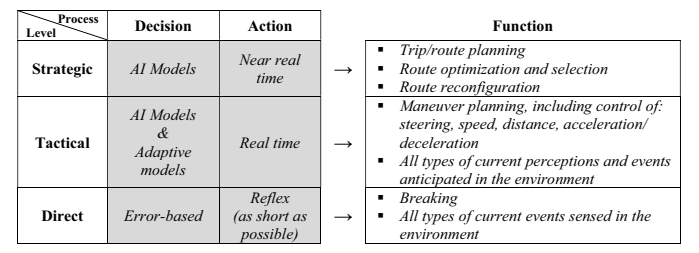
\includegraphics[width=\columnwidth]{Figures/literature_review/proposal/SystemFunctionality-3.png}
			\caption{Classes of ADAS and their Requirements for Decision and Execution~\cite{ionita_autonomous_2017}}
			\label{fig:adasFunctionsIonita}
		\end{figure}

	\subsection{Vision Technology and Techniques}
		When investigating how AVs handle blindspot handling compared to human drivers, the paper `Automated driving: Safety blind spots' by Ian Y. Noy~\cite{noy_automated_2018} suggests the current implementations within ADAS and compares it to standard driving errors. Although, the paper does not directly reflect on motorcycles, the paper details ADAS systems and how the transition from ADAS to AVs is possible. An important quote from the paper is that `AD technologies are suboptimal in that they fail to address critical blind spots and will likely lead to unnecessary losses and injuries because insufficient consideration is given to integrating the human element into overall sociotechnical road transportation system'~\cite{noy_automated_2018} suggests that transitioning from ADAS to AVs is relatively dangerous if blindspot judgements are overlooked. With further research in this area, it will provide more information to understand if AVs are safer than human drivers on the road.

		Light Detection and Ranging (LiDAR) uses a pulsed laser to gather information about the object surroundings, providing depth that images cannot capture. Within the paper, `Pedestrian recognition and tracking using 3D LiDAR for autonomous vehicle' by Heng Wang~\cite{wang_pedestrian_2017}, a quote ``LiDARs are another kind of commonly used sensors for pedestrian recognition, compared with cameras, LiDARs can provide accurate range information and larger field of view.''. Heng Wang points out that the use of LiDAR widens the field of view.
		
		After researching some extra information, it was found within the report `What Happens for a ToF LiDAR in Fog?'~\cite{li_what_2021} that the failure rate of detection in Diffuse Reflection Targets: 2.1\% and Retro-Reflective Objects: 0.7\% in the range of 0-10m, Diffuse Reflection Targets: 10.3\% and Retro-Reflective Objects: 1.1\% in the range of 10-15m, Diffuse Reflection Targets: 15.1\% and Retro-Reflective Objects: 1.1\% in the range of 15-20m, and Diffuse Reflection Targets: 19.5\% and Retro-Reflective Objects: 0.7\% in the range of 0-10m~\cite{royo_overview_2019}

		When investigating how AVs handle blindspot handling compared to human drivers, the paper `Automated driving: Safety blind spots' by Ian Y. Noy~\cite{noy_automated_2018} suggests the current implementations within ADAS and compares it to standard driving errors. Although the paper does not directly reflect on motorcycles, the paper details ADAS systems and how the transition from ADAS to AVs is possible. An important quote from the paper is that `AD technologies are suboptimal in that they fail to address critical blind spots and will likely lead to unnecessary losses and injuries because insufficient consideration is given to integrating the human element into overall sociotechnical road transportation system'~\cite{noy_automated_2018} suggests that transitioning from ADAS to AVs is relatively dangerous if blindspot judgements are overlooked. Further research in this area will provide more information to understand if AVs are safer than human drivers on the road.

	\section{Model Architectures}
		Yen-Yi Wu~\cite{wu_pedestrian_2016} suggests using a Deep Belief Networks (DBN) model for object classification. The model correctly classifies images: pedestrians, bikes, motorcycles and other vehicles. The model thrives an 89.53\% accuracy.

		The r-CNN model merges a CNN approached model with a Region-based model to create a deeper layered one. The aim is to increase accuracy and performance regarding object classification. The R-CNN uses a selective search algorithm to find certain features within the set of images and focus on the objects that match the specified features using diverse strategies. This approach means that when training the model, it is equally important to understand what the layers do and how they filter the image to change the test data to analyse the different performances and accuracies of the training and testing.~\cite{uijlings_selective_2013}~\cite{ren_faster_2015}

		DBN model is based on Restricted Boltzmann Machine (RBM) layers to train the model. According to `An overview on Restricted Boltzmann Machines'~\cite{zhang_overview_2018} explains that RBMs pre-train the networks' weights. This technique is done layer by layer and applies gradient descent methods to fine-tune the weights. This method alone allows the neural network to optimise the hyper-parameters, which in turn boosts accuracy and optimises the model's overall performance.

		Both model suggestions both use CNN, whether it is merging CNN or comparing to CNN. The Journal Article titled "Detection of Motorcyclists without Helmet in Videos using Convolutional Neural Network" by C. Vishnu includes a layer designed to recognise whether a motorcyclist is wearing a helmet. This finding emphasises an essential feature in ensuring the safety of riders on the road. Using a Convolutional Neural Network, the layer can accurately detect whether a helmet is being worn, which can help prevent accidents and reduce injuries. It is impressive to see how technology can enhance safety measures in everyday life. The layers proposed by the author should benefit the datasets used in this research project. The layer structure is fatigue, although it involves ReLU, max-pooling, fully connected and a loss function (Support Vector Machines or Softmax) layers.
        
        Figure~\ref{fig:adasFunctionsIonita} displays the DBN and RBM layers from the paper, `Parallel computing method of deep belief networks and its application to traffic flow prediction' illustrated by Lu Zhao~\cite{zhao_parallel_2019}. DBN is not a convolutional network compared to CNN. DBN consists of a two-layer graph, including a visible layer below and a hidden layer above, displayed in figure~\ref{fig:dbnRBMLayers}. The author and illustrator mention that the RBM layers illustrated are slightly different to the classical Boltzmann Machine.~\cite{zhao_parallel_2019}

		\begin{figure}[htp]
			\centering
			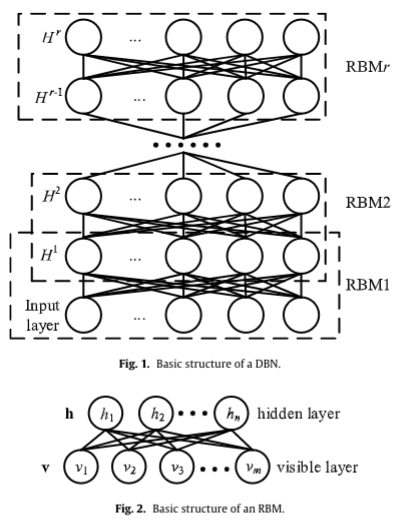
\includegraphics[width=\columnwidth]{Figures/literature_review/proposal/DBNRBMLayers.png}
			\caption{DBN and RBM Model Layers~\cite{zhao_parallel_2019}}
			\label{fig:dbnRBMLayers}
		\end{figure}

	\section{Datasets and Preparation Idealogies}
		Finding the suitable dataset for the given research question involves first identifying the required information. The requirements of the dataset need to have motorcycles on the road with different situations, camera angles and visibility. After exploring through some datasets, three image classification datasets, `TuSimple'~\cite{jeong_end--end_2017}, `Car vs Bike Classification'~\cite{deepnets_car_nodate} and `MB10000'~\cite{espinosa_motorcycle_2018}. The ideal datasets at the time was `TuSimple'. However, the dataset was twenty-five gigabytes, and meant that training the dataset was too much for individual research. The `Car vs Bike Classification' dataset lacked authentic motorcycle and car images in realistic situations. However, the dataset was lightweight, with one hundred and eight megabytes. These mentioned specifications meant that the `MB10000' had an optimistic fitness to support this experiment. The dataset has realistic situations, motorcycles with other vehicles and image sequences to support image classification. The dataset has four-hundred and twenty-six megabytes of filesize.

		`Pedestrian, Bike, Motorcycle and Vehicle Classification via Deep Learning: Deep Belief Network and Small Training Set' by Yen-Yi Wu~\cite{wu_pedestrian_2016} goes over different visibility levels that affect pedestrians, bikes, motorcycles and vehicles and how image classification affects these vehicles. The image preprocessing involves converting colour images to greyscale. Including edge emphasis, detection to enhance to the image, with the fundamental aim to detect edges of objects seamlessly. The paper suggests using a fixed threshold and Otsu methods to threshold greyscale images and use bilinear interpolation for image resizing. These methods should increase the visibility of the objects within the images are good notes for when conducting any experiments.

\chapter{Research Methodology}
\label{chap:researchMethodology}

\chapter{Reflection}

\chapter{Terminology}
List of terminologies used in this document:-
\begin{itemize}
	\item .
\end{itemize}

%----------
%	Bibliography
%----------	

\clearpage
\nocite{*}
\small{\bibliographystyle{IEEEtran}
	\bibliography{ref}}

%----------
%	Appendix
%----------	

% If your work includes Appendix, you can uncomment the following lines
%\chapter* {Appendix x}
%\pagenumbering{gobble} % Appendix pages are not numbered

\end{document}